% vim: fo=aw2tq tw=100 spell
\chapter{Functional Overview}

\begin{nowordcount}
\begin{figure}[htbp]
\centering
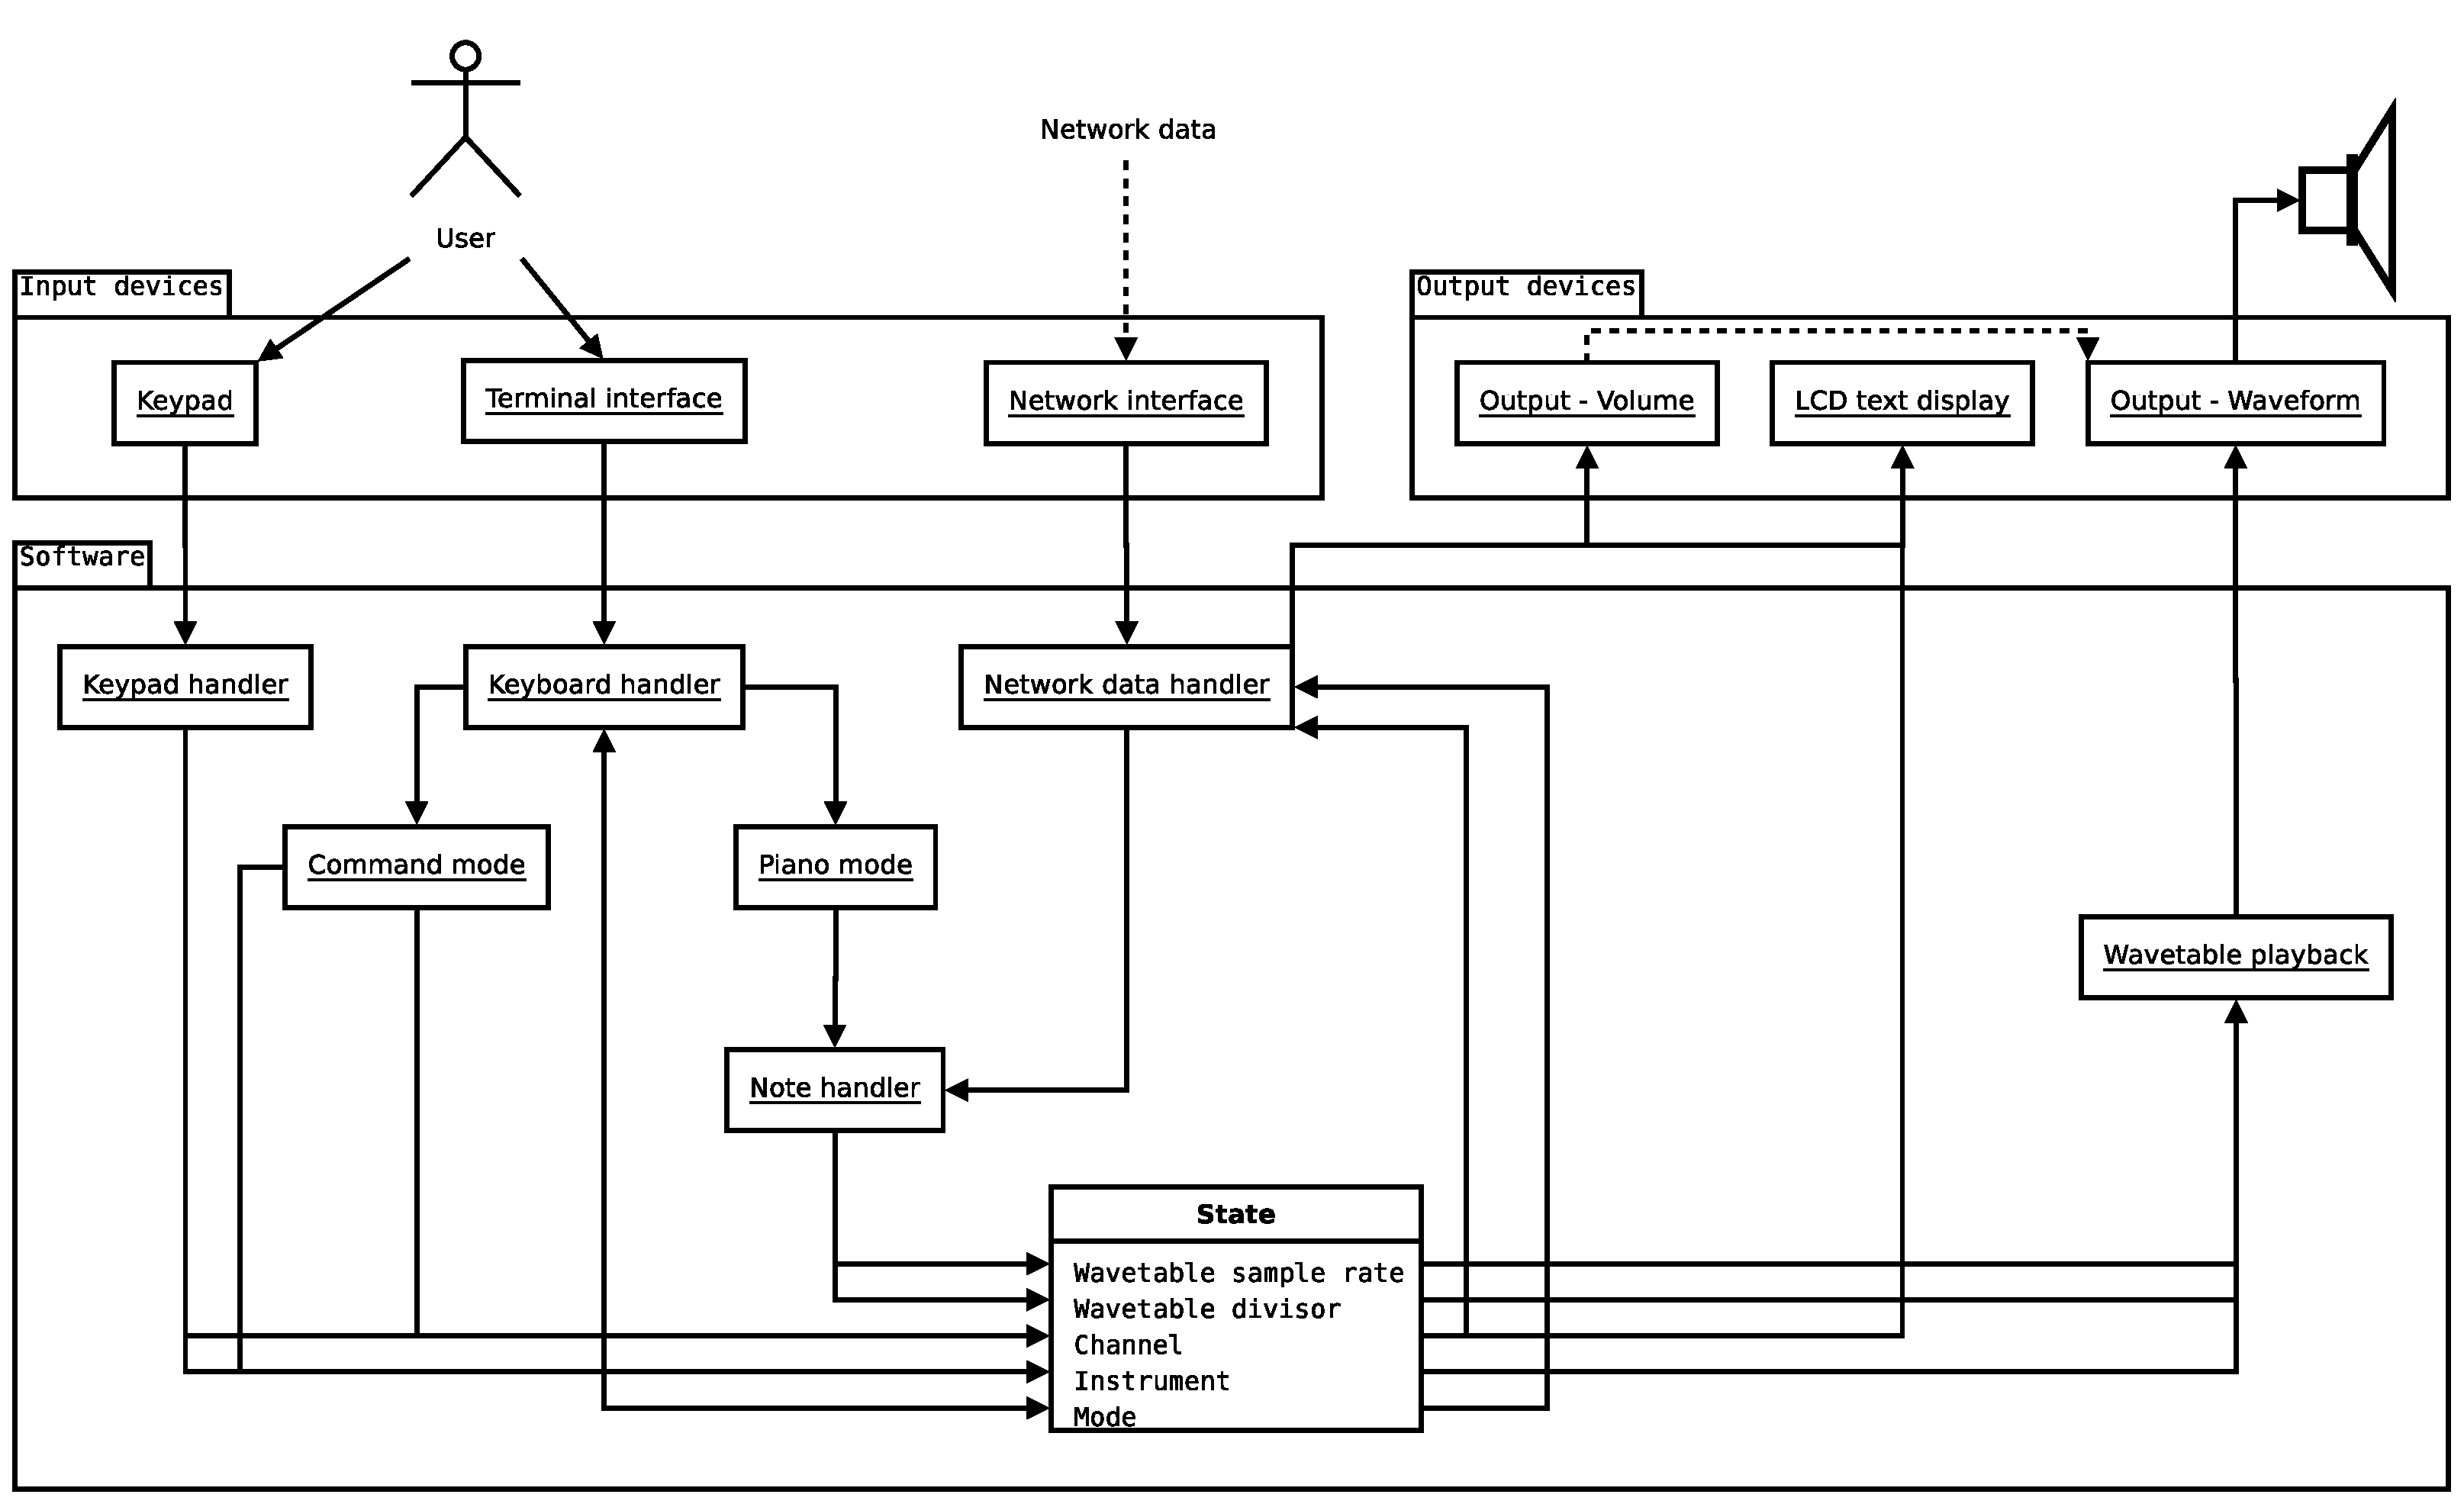
\includegraphics[totalheight=0.55\textheight,angle=90]{images/overview}
\caption{System Overview}\label{fig:systemoverview}
\end{figure}
\end{nowordcount}

The diagram in Figure \ref{fig:systemoverview} shows the conceptual architecture of my system.  The 
basic idea is that various inputs are processed and in some way modify the state of the system, and 
this state in turn affects the operation of the continuously-running wave table playback.

\section{Network Interface}
\label{sec:overview:network}

The network interface is a serial connection which receives a data stream at a rate of one 34-byte 
packet every $34ms$.  The data format is sixteen pairs of bytes, each pair containing a MIDI note 
value and a volume level (both in the range 0--127), with each pair representing a channel between 0 
and 15 (in order).  The packet is terminated with a null byte (00h) and a carriage return (0Dh).  
The mapping of channel identifiers to instruments is shown in Table \ref{tab:channelids}.  For the 
``Percussion'' channel, the volume level represents the particular percussion instrument to play 
rather than the volume at which to play it.

\begin{nowordcount}
\begin{table}[htbp]
\centering
\begin{tabular}{c | l}
ID & Instrument \\
\hline\hline
0 & Bass Guitar \\
1 & Cello \\
2 & Church Organ \\
3 & Piano \\
4 & Saxophone \\
5 & Melody \\
6 & Violin \\
7 & Trombone \\
8 & Trumpet \\
9 & French Horn \\
10 & Synth \\
11 & Electric Guitar \\
12 & Acoustic Guitar \\
13 & Flute \\
14 & Piccolo \\
15 & Percussion
\end{tabular}
\caption{Network data channels}\label{tab:channelids}
\end{table}
\end{nowordcount}

The network handler collects data from the incoming byte stream.  The bytes are counted, and the 
currently selected channel is used to decide which note/volume pair to store (see 
Section~\ref{sec:design:network-handler} for rationale on this design).  When the end of a packet is 
detected, the byte count is checked and the data discarded if the packet was incomplete.  The packet 
is also discarded if the system is not in ``network mode'' (see Section~\ref{sec:overview:state}).
If there is no reason to discard the packet, the data is used to set the state of the system.  The 
volume is converted to an 8-bit value (left-shifted) and output to the hardware, and also used to 
set the appropriate part of the LCD text display.  The note handler is run with the note value.

\section{Note Handler}
\label{sec:overview:note-handler}

The note handler ``receives'' a MIDI note value, and uses it to find the appropriate state 
information in a lookup tables.  Firstly, a playback lookup table is used to find the PRT value and 
divisor, which are written to the PRT reload register and divisor register used by the playback loop 
respectively.  Secondly, a display lookup table is used to find a 4-character representation of the 
note, which is written to the LCD text display.  See Section~\ref{sec:design:lookup-tables} for 
details of the lookup tables.

\section{Wavetable Playback}
\label{sec:overview:playback}

Wavetable playback is controlled by the PRT and divisor settings --- how these affect the note being 
played is explained in Section~\ref{sec:design:wavetables}.  Every time the playback routine is 
called, the next sample from the wavetable for the current instrument is sent to the output device.  
The PRT reload value controls how often the playback routine is called.  The ``divisor'' controls 
the step between samples --- for example, 1 means every sample, 3 means every third sample.  The 
wavetable playback is affected only by the state of the system, it is not directly called from 
anywhere.

\section{Keypad Handler}
\label{sec:overview:keypad}

Since the keypad has 16 possible values, when a button is pressed on the keypad, the value is used 
to set the channel and instrument selection to that value.  \todo{Expand this?}

\section{Terminal Interface}
\label{sec:overview:terminal}

The SBC is connected to a PC via a serial connection.  This allows the user to interact with the 
software over this connection using terminal software, such as Seyon.  The user interface provided 
over the serial terminal is purely additional functionality --- the essentials of playback and 
channel selection can be used without this interface.  The keyboard handler decides what should be 
done based on the mode and the key pressed.

\begin{figure}
\centering
\includegraphics[width=0.9\textwidth]{images/terminal-prompt}
\caption{Serial Terminal Prompt}\label{fig:terminal-prompt}
\end{figure}

\subsection{``Network Mode''}

In the default mode, there are three possible actions the user can perform 
(Figure~\ref{fig:terminal-prompt}):

\begin{description}
\item[Change instrument:] Change the current instrument without changing the channel being read.  
This is useful for demonstrating all of the instruments when not all channels have activity.
\item[Change channel:] Change the current channel without changing the instrument.  Useful for 
testing all of the channels when only one instrument sample has been loaded, also makes sense for 
this to be possible given the availability of the first action.
\item[Piano mode:] Enter piano mode, where keyboard input is mapped to changing the note.
\end{description}

\subsection{``Piano Mode''}

In piano mode, the currently selected octave combined with pressing a key determines the note to 
play (explained further in Section~\ref{sec:design:piano-mode}).  Figure~\ref{fig:piano-mode} shows 
how the keys are mapped --- the layout is based on the note layout on a piano.  Since there are four 
rows of normal characters on a standard keyboard I decided to map the current octave and the octave 
above.  The ``$+$'' and ``$-$'' keys can be used to change the current octave.  Pressing ``Ctrl+D'' 
exits piano mode, returning to network mode.

When a note key is pressed, the correct MIDI note is found (via lookup tables and the octave offset) 
and passed to the note handler (Section~\ref{sec:overview:note-handler}).

\begin{figure}
\centering
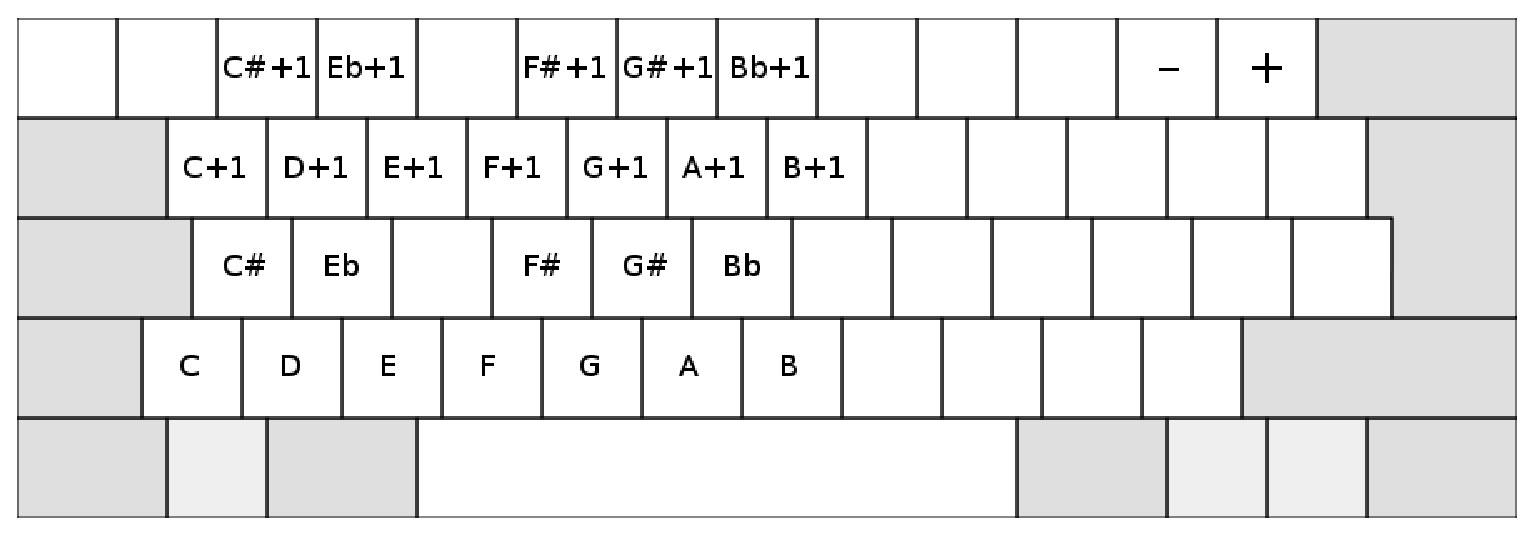
\includegraphics[width=0.9\textwidth]{images/piano-mode}
\caption{``Piano Mode'' Keyboard Layout}\label{fig:piano-mode}
\end{figure}

\section{State}
\label{sec:overview:state}

There are 5 main elements to the state of the system:

\begin{description}
\item[Wavetable sample rate:] The rate at which samples are read from the instrument wavetable and 
output.  This takes the form of the PRT reload value, and is one of two factors affecting the 
generated note frequency.
\item[Wavetable divisor:] The step size when reading from the instrument wavetable.  This is the 
second factor affecting the note frequency.  How these affect the frequency is explained in 
Section~\ref{sec:design:wavetables}.
\item[Channel:] The current channel being played.  This affects which data is used from the network 
stream, and the channel name being displayed on the LCD text display.
\item[Instrument:] The current instrument being used.  This affects which wavetable sample is being 
used by the playback routine.
\item[Mode:] The current system mode --- ``network'' or ``piano''.  This affects the actions of key 
presses on the terminal, and also whether or not network data is ignored.
\end{description}
